\documentclass[a4paper, twocolumn]{article}
\usepackage[pdftex, hidelinks,
            pdftitle={Report},
            pdfauthor={Erik S. Vasconcelos Jansson},
            pdfsubject={Report},
            pdfkeywords={report}]{hyperref}

\usepackage{bm}
\usepackage[T1]{fontenc}
\usepackage[utf8]{inputenc}
\usepackage{algorithmic}
\usepackage{algorithm}
\usepackage{amsfonts}
\usepackage{booktabs}
\usepackage{amssymb}
\usepackage{courier}
\usepackage{booktabs}
\usepackage{graphicx}
\usepackage{listings}
\usepackage{mathtools}
\lstset{basicstyle=\footnotesize\ttfamily,
        breakatwhitespace = false,
        breaklines = true,
        keepspaces = true,
        language = C++,
        showspaces = false,
        showstringspaces = false,
        belowcaptionskip = \bigskipamount,
        framerule = 0.80pt,
        frame = tb,
        numbers = left,
        belowskip = \bigskipamount,
        escapeinside={<@}{@>}}

\title{Introduction to Machine Learning \\
       Individual Laboration Report --3--}
\author{{Erik Sven Vasconcelos Jansson} \\
        {\href{mailto:erija578@student.liu.se}
        {\texttt{erija578@student.liu.se}}} \\
        {Linköping University, \, Sweden}}

\begin{document}
    \pagenumbering{arabic}
    \maketitle % Titles...

    \section*{Assignment 1}

        Now that \emph{linear regression} and \emph{cross-validation} have been studied for \emph{regression problems} (involving continuous target variables), the question is how to apply the same concept to \emph{classification problems} (which involve a discrete amount of target variables). Both \emph{Linear Discriminant Analysis (LDA)} and \emph{Logistic Regression} can be used to achieve this, and also to draw \emph{decision boundaries}.

        In this task the goal is to \emph{classify} the \emph{Sex} of \emph{Australian Crabs} by using their \emph{Carapace Length} and \emph{Rear Width} using \emph{LDA} and thereafter plotting the \emph{decision boundary}. Plotting the data gives Figure~\ref{fig:crabs}. As can be seen, a decision boundary seems to exist.

        Firstly, the \emph{linear parameters} $w_0$ and $\bm{w}$ need to be found for each class $k$, essentially creating our \emph{target hypothesis function} for each one of these $k$. Finding these parameters is done with Equations~\ref{eq:lda}, essentially computing the mean $\bm{\hat{\mu}}_k$ for each class $k$ which is used to derive the \emph{covariance matrices} $\Sigma_k$.

        \begin{equation} \label{eq:lda}
        \begin{split}
            \hat{\pi}_k &= \frac{N_k}{N} \\
            \hat{\mu}_k &= \frac{1}{N_k}\sum_{i \in k}{\bm{x}_i} \\
            \Sigma_k &= \frac{1}{N_k}\sum_{i \in k}{(\bm{\hat{\mu}}_k - \bm{x}_i)(\bm{\hat{\mu}}_k - \bm{x}_i)^\intercal} \\
            \hat\Sigma &= \frac{1}{N}\sum_{k \in K}{N_k \Sigma_k} = \sum_{k \in K}{\frac{\mathrm{cov}\,X_k}{|X_k|}}
        \end{split}
        \end{equation}

        \begin{equation} \label{eq:weights}
        \begin{split}
            w_{k} &= -\frac{\bm{\hat\mu}_k^\intercal}{2}\hat\Sigma^{-1}\bm{\hat\mu}_k + \log\hat{\pi}_k \\
            \bm{w}_{k} &= \hat\Sigma^{-1}\bm{\hat\mu}_k
        \end{split}
        \end{equation}

        Finally, computing $\hat{\Sigma}$ is done by using these $\Sigma_k$, which is thereafter used to calculate $w_0$ and $\bm{w},\, \forall k$. Implementation of these formulae in \emph{R} can be found in Listing~\ref{lst:lda} under lines \texttt{15-39} i the \texttt{lda} function. All equations are in \emph{Friedman et al's}~\cite{friedman2009elements} book.

        \begin{equation} \label{eq:discfun}
        \begin{split}
            \delta_k(\bm{x}) &= w_0 + \bm{w}
        \end{split}
        \end{equation}

        Using the \emph{Discriminant Function} in Equation~\ref{eq:discfun} above, one can plot the line through each class $k$. The \emph{decision boundary} is in-between these 2 lines. In lines \texttt{58-61} we calculate the \emph{intercept} and the \emph{slope} of the \emph{decision boundary}, which gives us all the information needed to produce a new Figure~\ref{fig:boundarylda}. The fit seems perfect, exactly as previous Figure~\ref{fig:crabs}.

        \begin{figure}[h!]
            \centering
            \caption{Sex Classifications of Australian Crabs}
            \label{fig:crabs}
            \includegraphics[width=0.45\textwidth]{share/crabs.eps}
        \end{figure}

        \clearpage

        Thereafter, by using \emph{Logistic Regression} instead, Figure~\ref{fig:boundarylr} can be obtained, which is a bit different...

        \begin{table}[h!]
        \begin{center}
        \begin{tabular}{lcc}
            \toprule
                \textbf{Class} & $w_0$ & $\bm{w}$ \\
            \midrule
                Female & -22.42 & (-2.161, 8.248) \\
                Male & -12.42 & (-0.213, 2.565) \\
            \bottomrule
        \end{tabular}
        \end{center}
        \caption{Predicted Parameters for Australian Crab}
        \label{table:parameters}
        \end{table}

        \begin{figure}[h!]
            \centering
            \caption{Crab Sex Decision Boundary using LDA}
            \label{fig:boundarylda}
            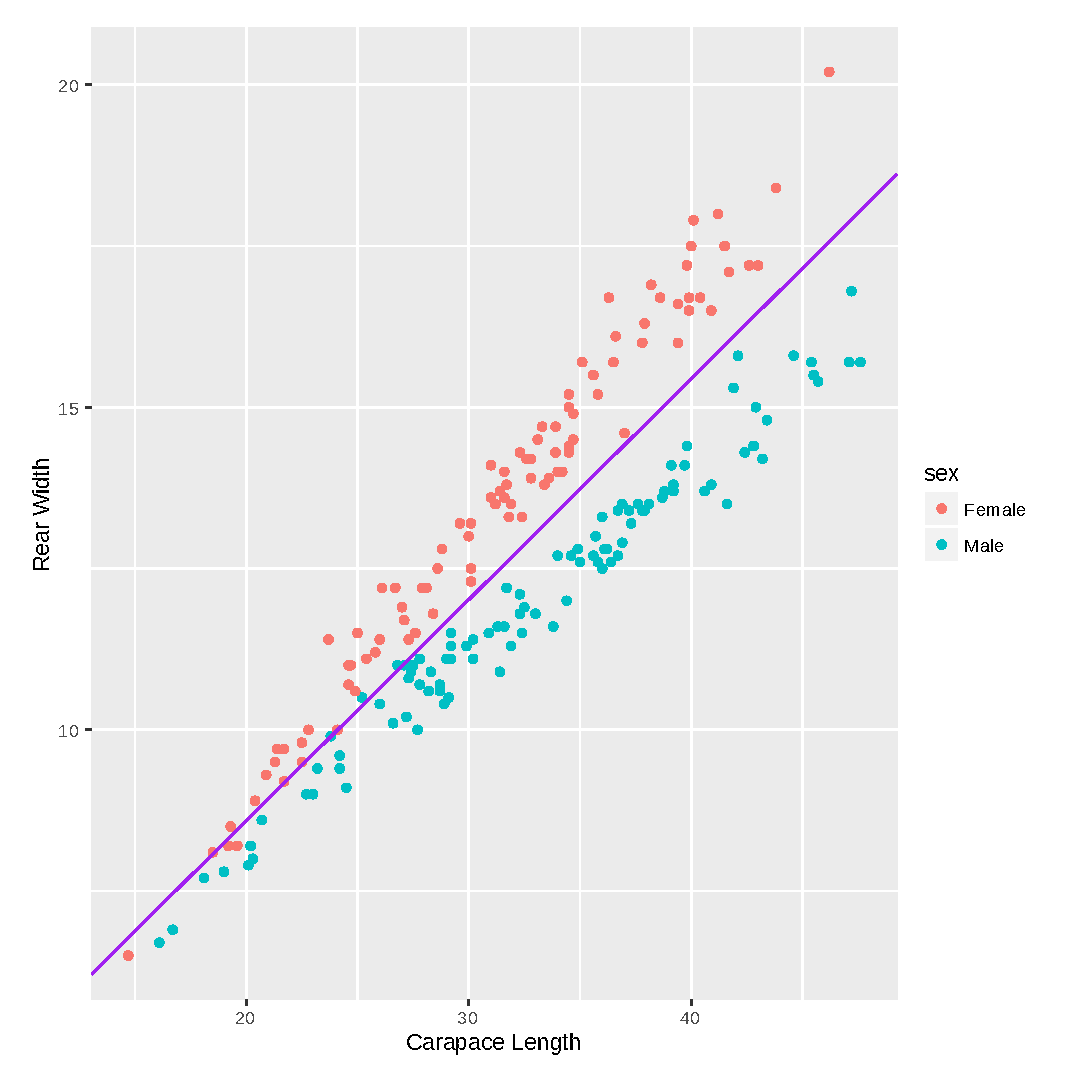
\includegraphics[width=0.44\textwidth]{share/boundary.eps}
        \end{figure}

        \begin{figure}[h!]
            \centering
            \caption{Crab Sex Decision Boundary using LR}
            \label{fig:boundarylr}
            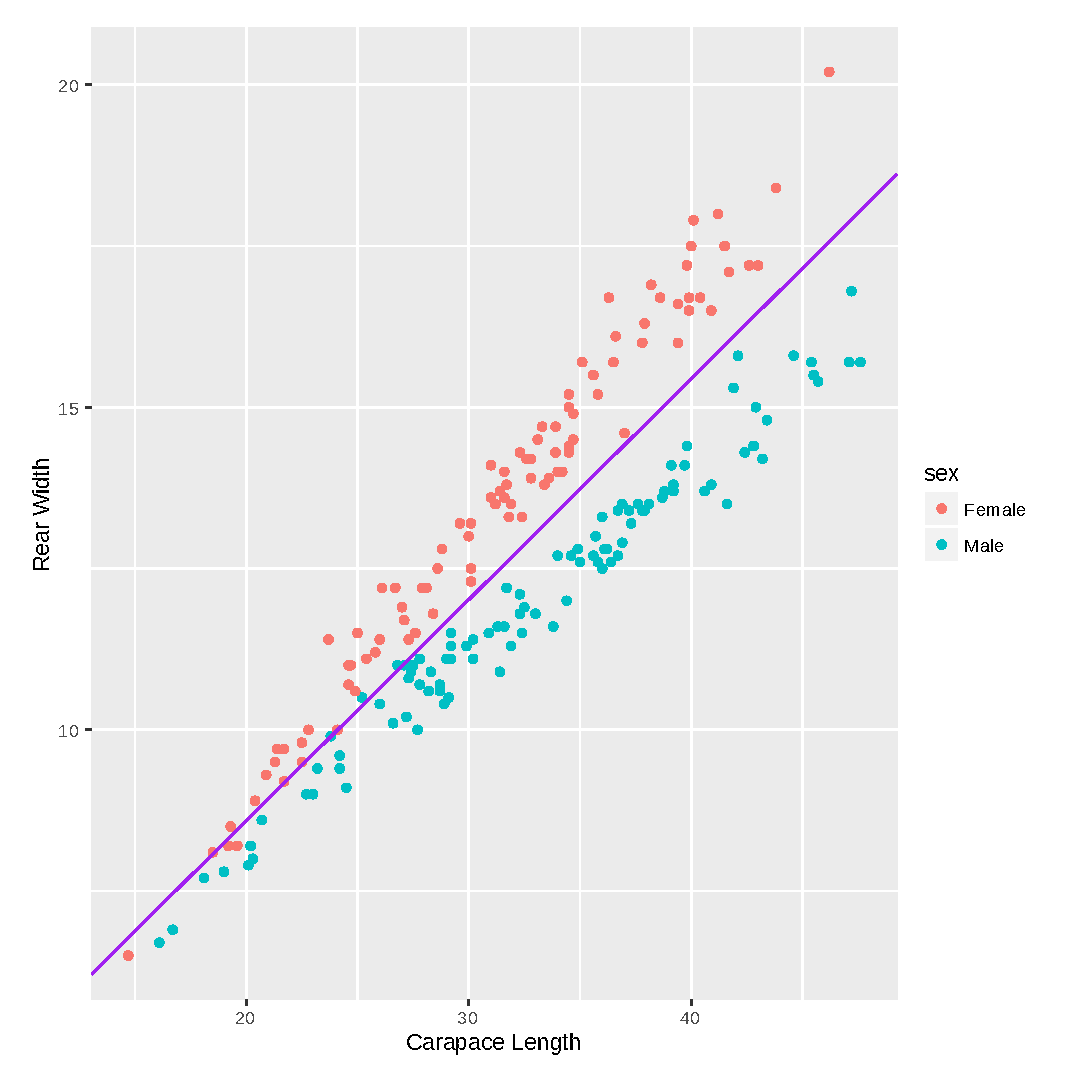
\includegraphics[width=0.44\textwidth]{share/boundary.eps}
        \end{figure}

        \newpage

    \section*{Assignment 2}

        \begin{figure}[h!]
            \centering
            \caption{Training and Validation Deviance Values}
            \label{fig:deviance}
            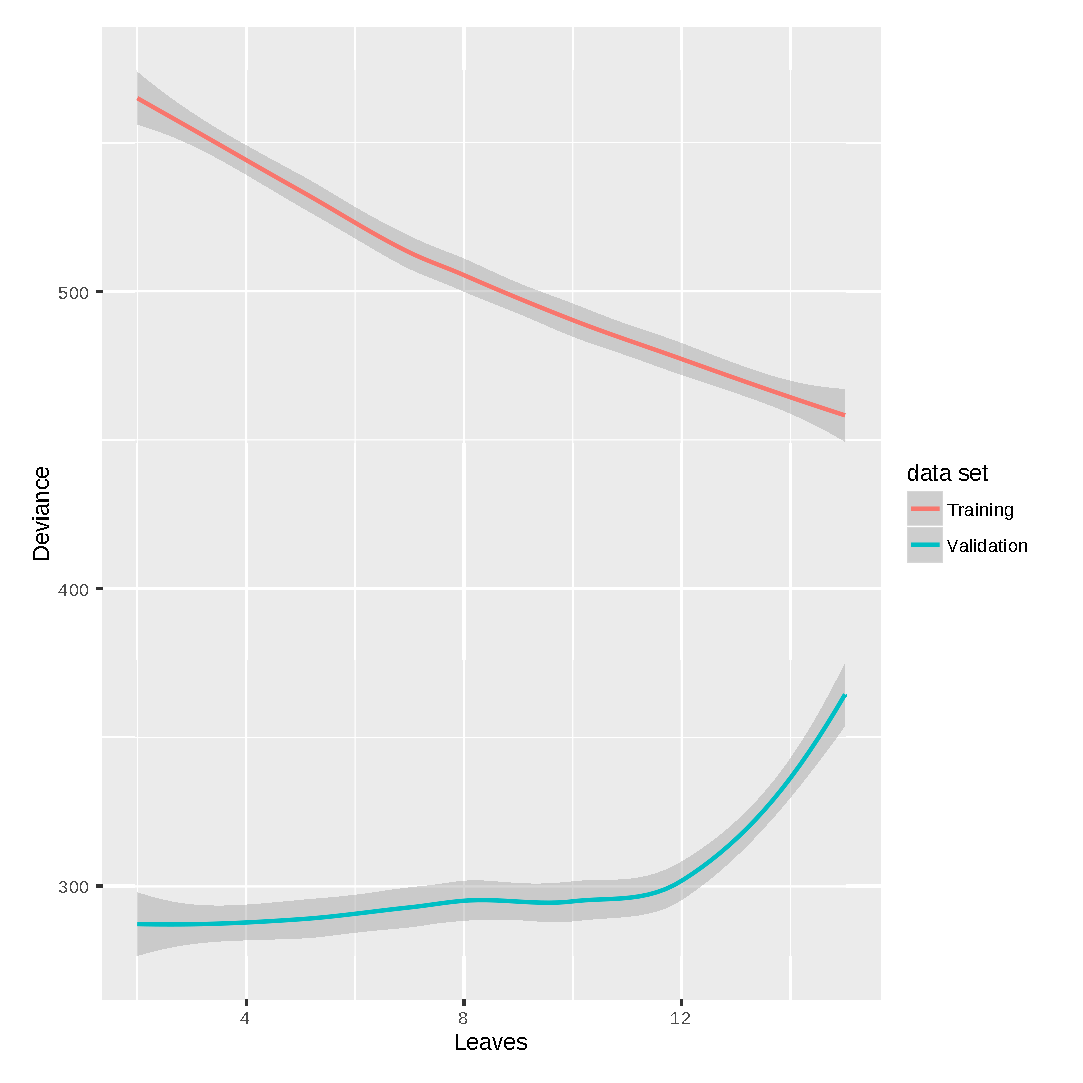
\includegraphics[width=0.5\textwidth]{share/deviance.eps}
        \end{figure}

    \clearpage \nocite{*}
    \bibliographystyle{alpha}
    \bibliography{report}

    \onecolumn \appendix
    \section*{Appendix}

    \lstinputlisting[caption={Linear Discriminant Analysis Assignment},label={lst:lda}]{../share/lda.r}
    \lstinputlisting[caption={Decision Trees and Na{\"\i}ve Bayes Assignment},label={lst:script}]{../share/script.r}

\end{document}
